\chapter{RESULT}
\patchcmd{\chapter}{\thispagestyle{fancy}}{}{}
\hrulefill\\
\thispagestyle{empty}

\section{Result}
The suggested AI-based resume analysis system is tested
by putting it into action and showing the results. The system
shows that it works by processing resumes, getting useful
information from them, and making smart suggestions.




\subsection{Input resume 1}:

\vspace{6pt}
\noindent The system can read resumes that are in PDF or DOCX
format. Fig 5 shows an example of a resume that was sent
to the system. The input has unstructured text that includes
personal information, skills, education, and work history.

\begin{figure}[ht]
\centering
 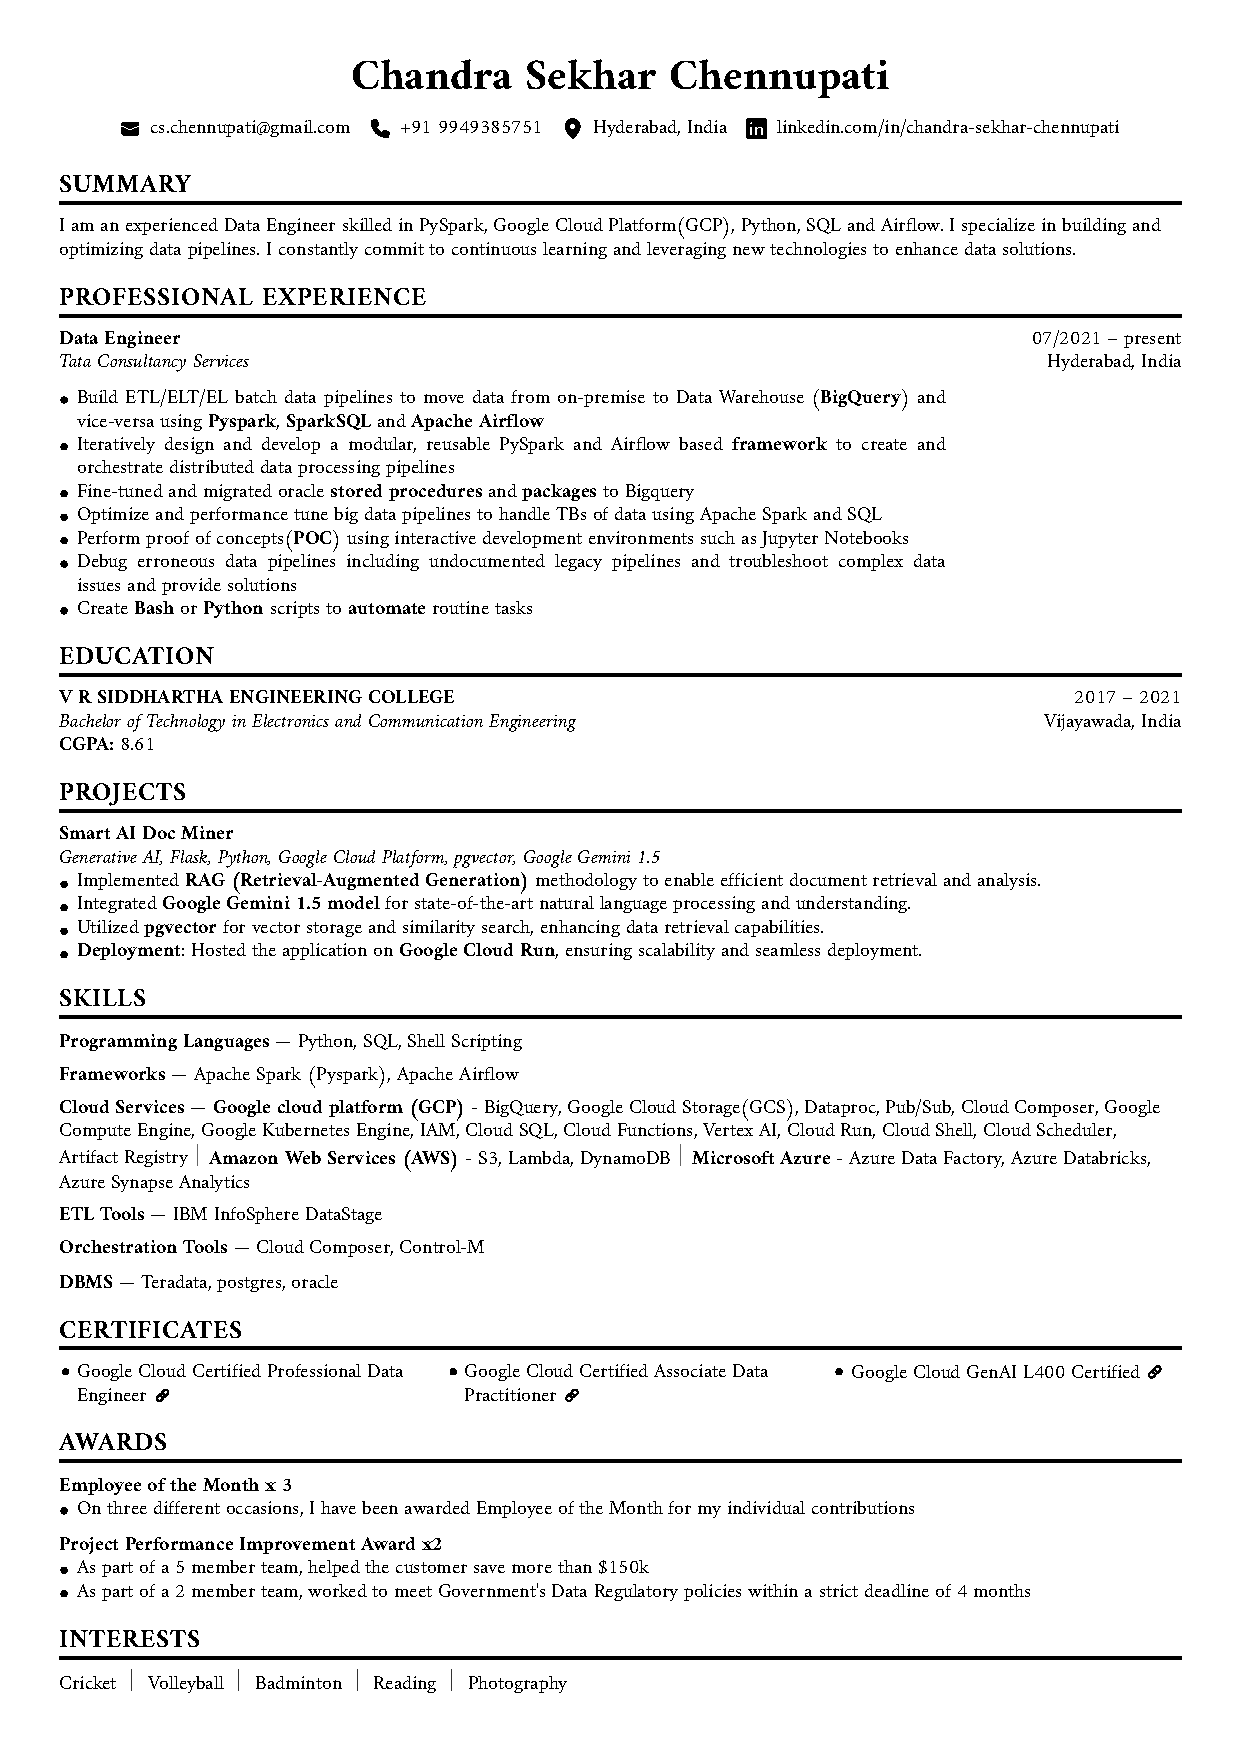
\includegraphics[width=0.8\textwidth]{images/anna resume.pdf}
 \captionof{figure}{Resume 1}
\end{figure}


\subsection{User Interface for Resume Upload}:

\vspace{6pt}
\noindent A user-friendly front-end interface lets users upload resumes
and start the analysis process. The system can read files in PDF
and DOCX formats, so you can use a variety of input types.
Once the resume is uploaded, it is processed automatically
without anyone having to do anything. Fig 5.3 shows the
screen where users choose and upload resumes for analysis.
The design makes it easy to get around and find results quickly,
which improves the overall user experience.


\begin{figure}[ht]
\centering
 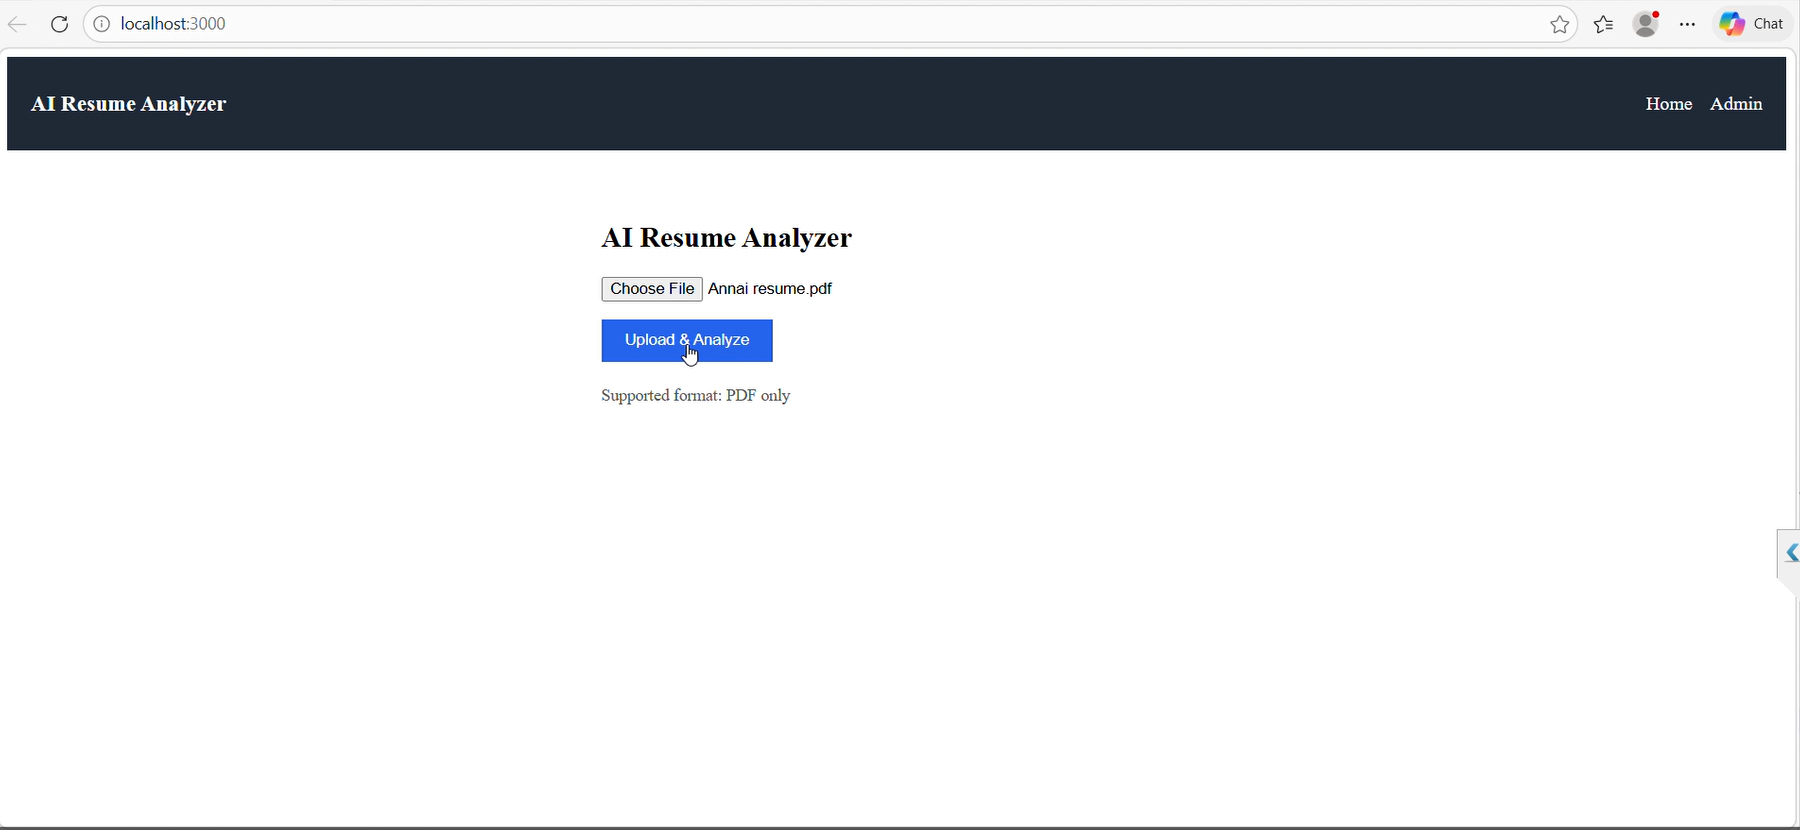
\includegraphics[width=1.3\textwidth]{images/otp1.png}
 \captionof{figure}{Dashboard Page}
\end{figure}

\begin{figure}[ht]
\centering
 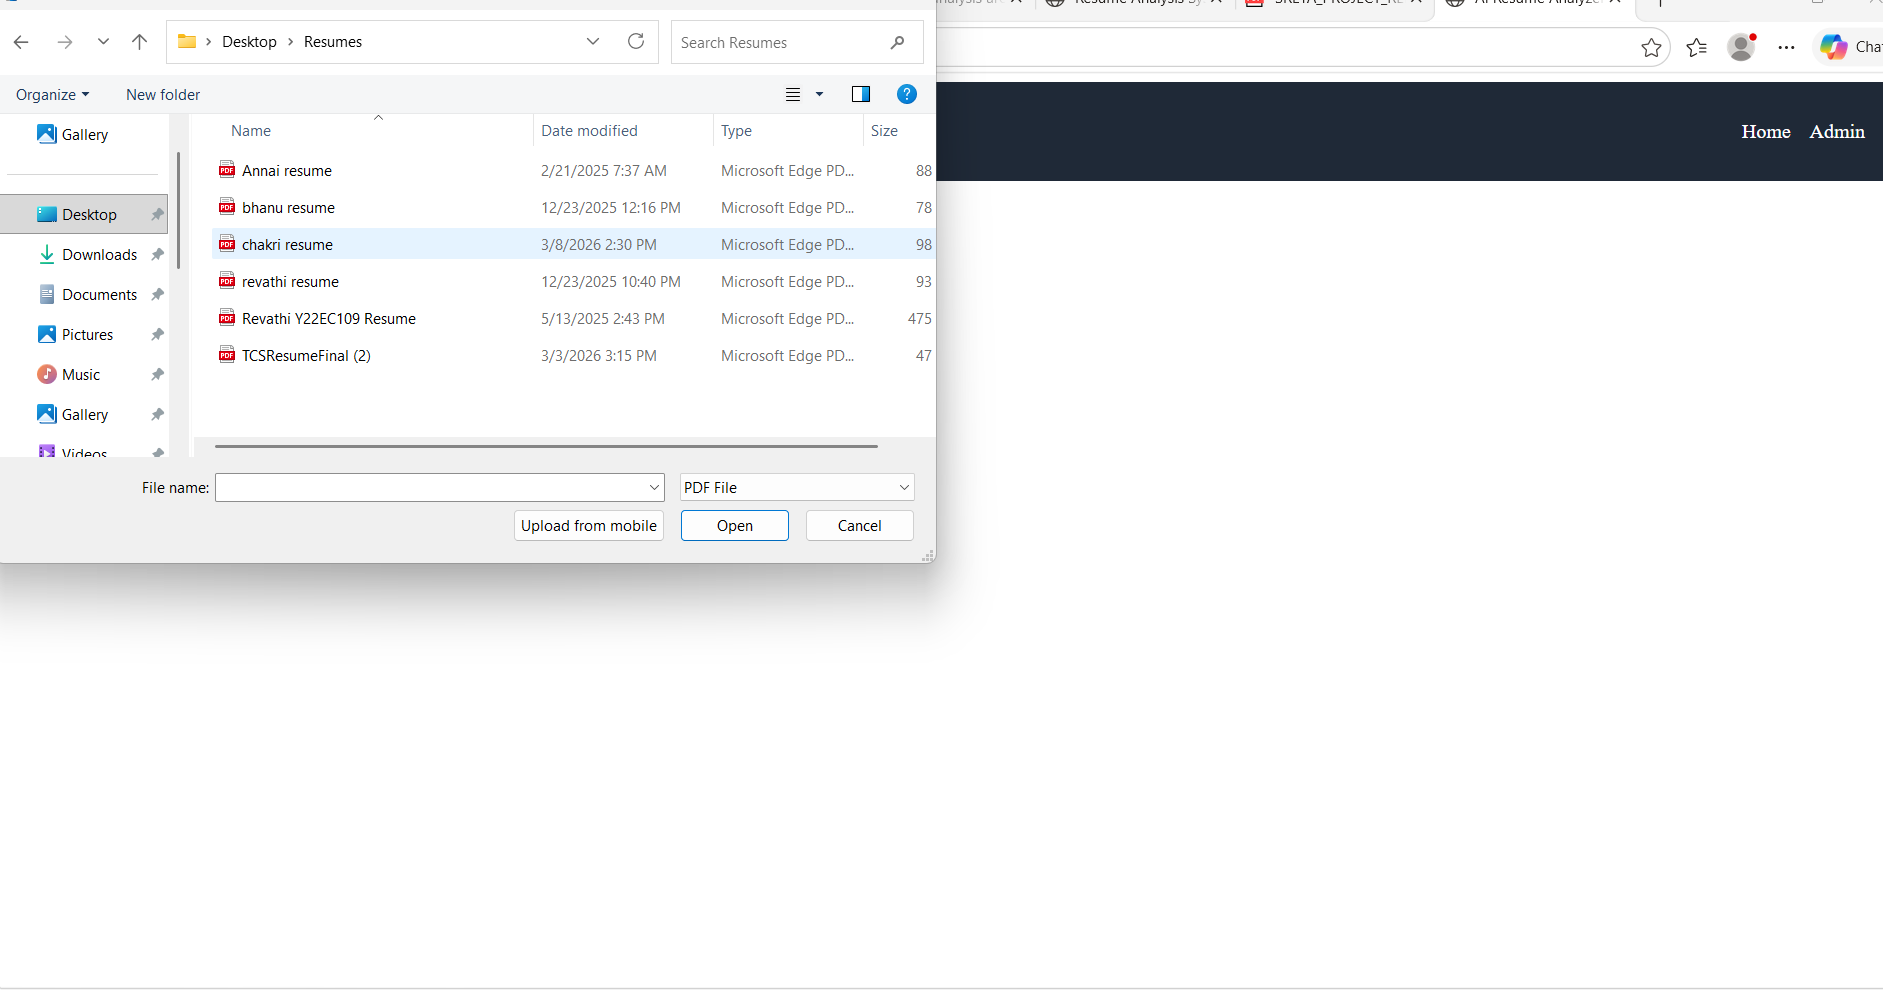
\includegraphics[width=0.8\textwidth]{images/otp12.png}
 \captionof{figure}{Uploading Resume}
\end{figure}



\subsection{Feature-Based Performance Analysis}:

\noindent The system looks at different factors, like skills, education,
work experience, and projects. Fig 5.6 shows these features
in a graph, showing how they affect the overall score. This
helps you figure out what parts of the resume are good and
what parts need work.
\begin{figure}[ht]
\centering
 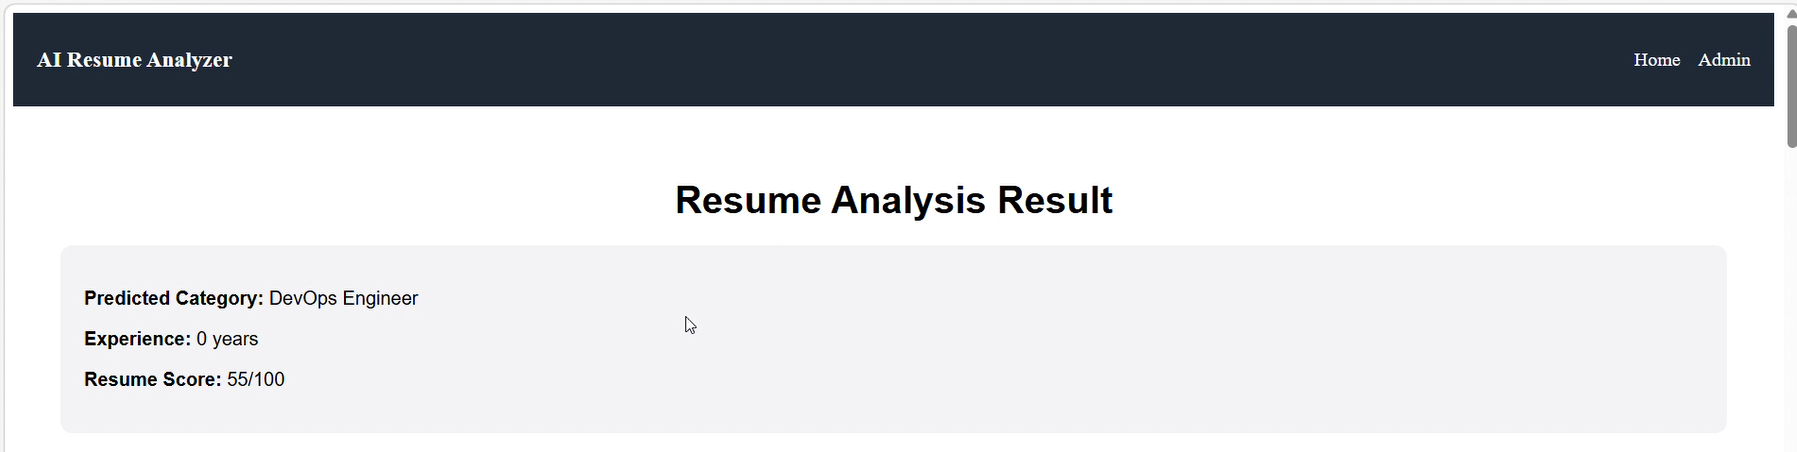
\includegraphics[width=0.8\textwidth]{images/otp 1-2.png}
 \captionof{figure}{ATS Score}
\end{figure}

\subsection{Extracted Skills and Recommendations}:
\noindent The NLP and NER modules pull out the relevant skills from
the resume. Fig 5.7 displays the extracted skills alongside
suggested skills and preparation guidelines. The system finds
weak or missing areas and gives suggestions for how to make
them better.

\begin{figure}[ht]
\centering
 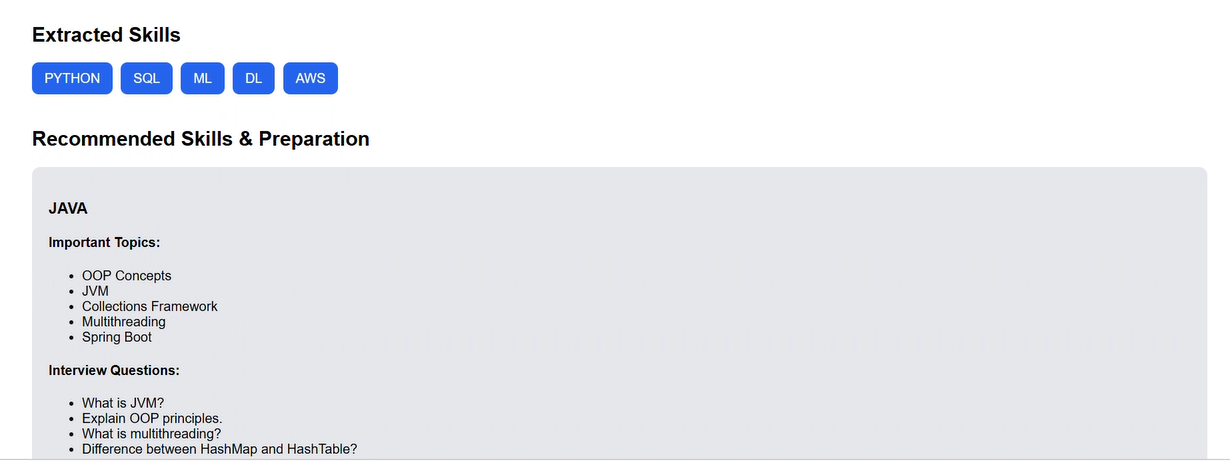
\includegraphics[width=1.0\textwidth]{images/otp 3.png}
 \captionof{figure}{Suggested Skills}
\end{figure}

\begin{figure}[ht]
\centering
 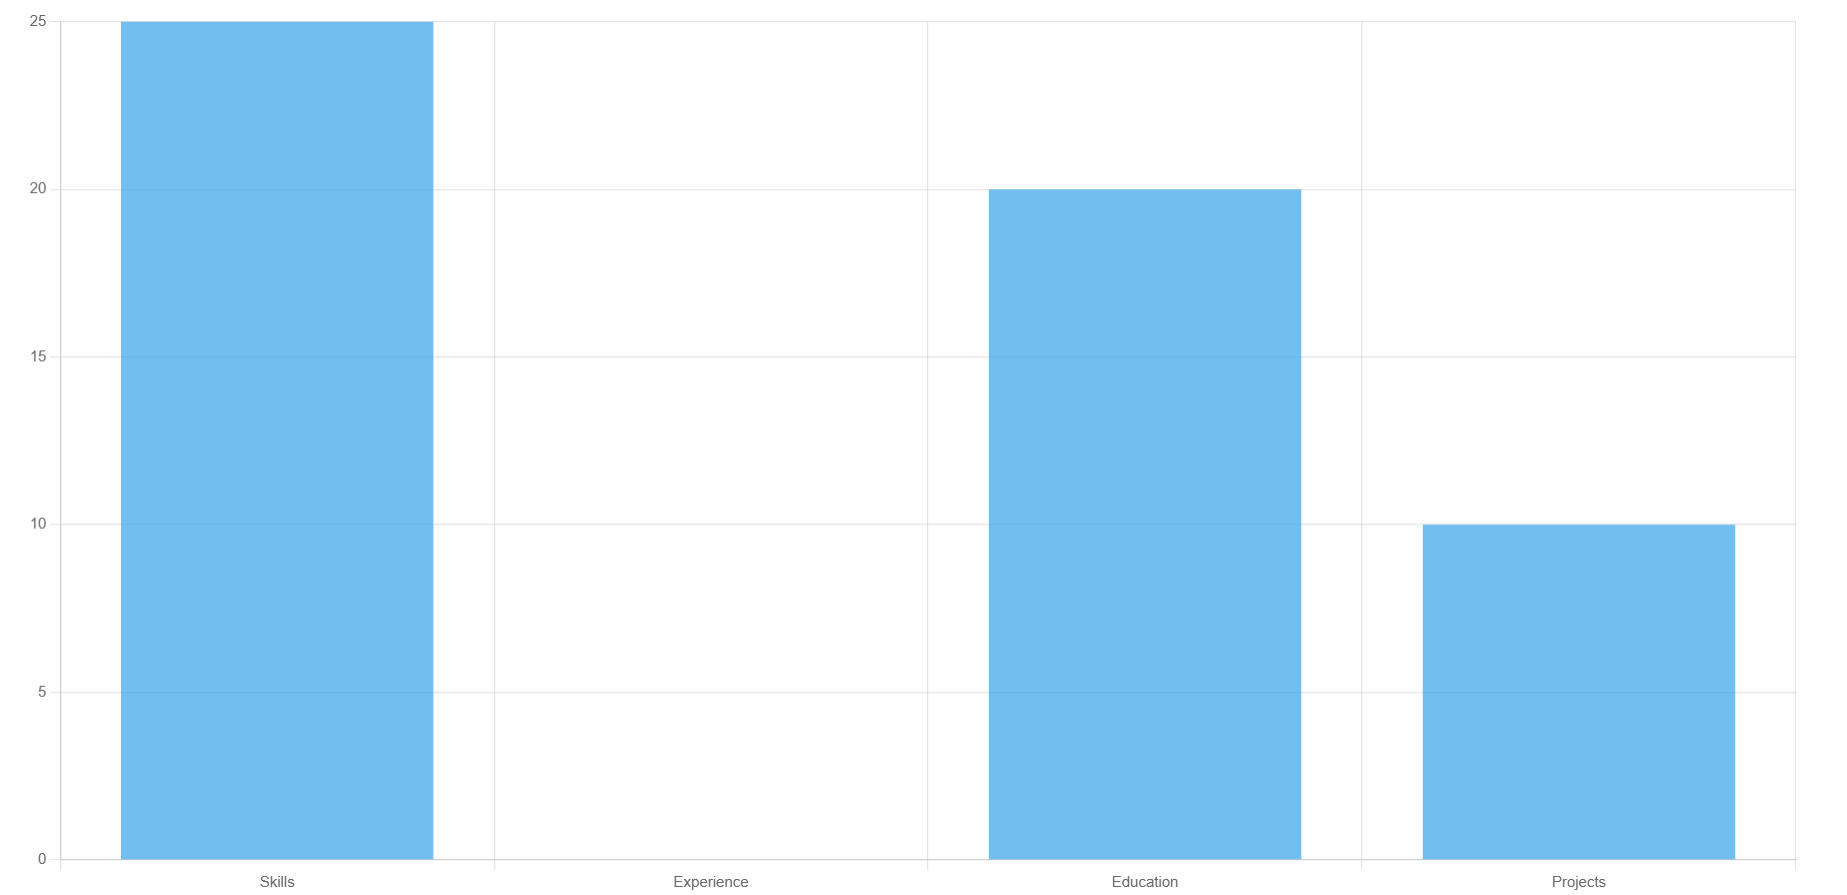
\includegraphics[width=0.8\textwidth]{images/otp2.png}
 \captionof{figure}{Scoring Graph}
\end{figure} 
\subsection{Domain-Specific Recommendations}:

\noindent The system makes recommendations based on the candi
date’s profile and the domain. Extracted Skills and Recommendations
topics and questions for Data Science interviews. These sug
gestions help candidates meet the standards of the industry.

\begin{figure}[ht]
\centering
 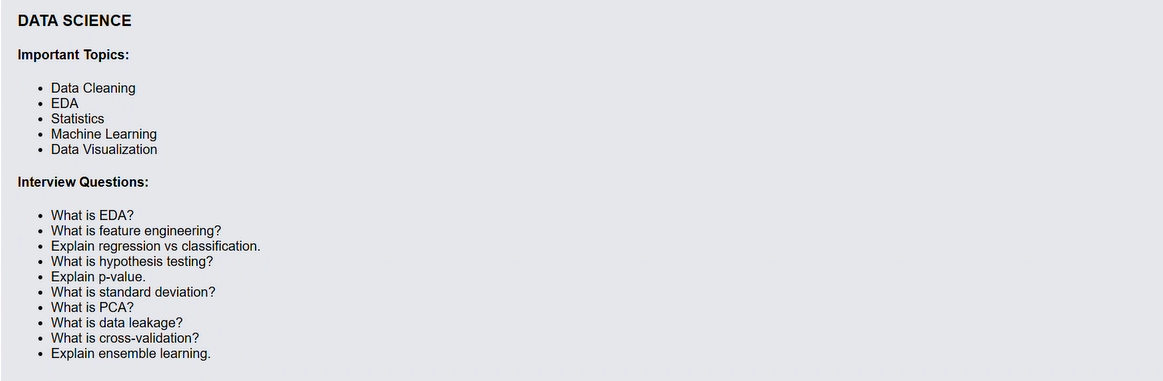
\includegraphics[width=1.0\textwidth]{images/otp 4.png}
 \captionof{figure}{Mock Interview Questions}
\end{figure}



\begin{figure}[ht]
\centering
 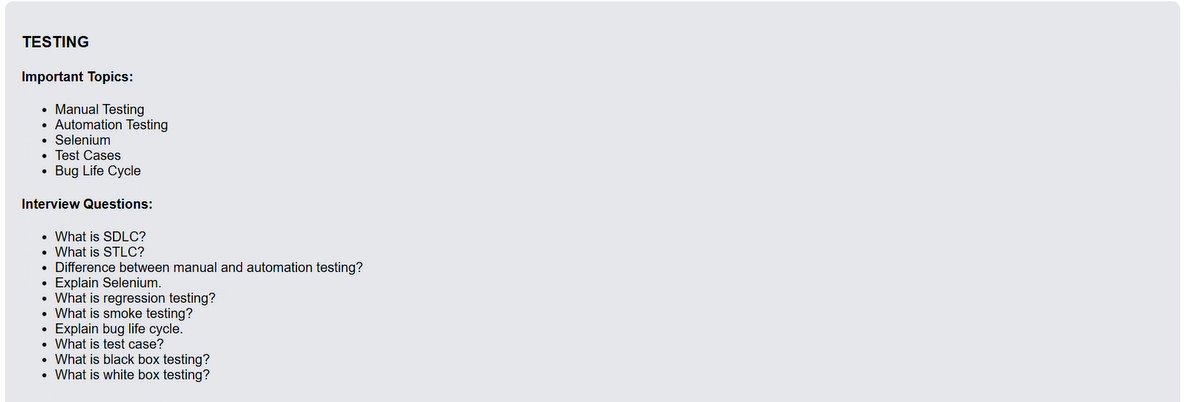
\includegraphics[width=1.0\textwidth]{images/otp 6.png}
 \captionof{figure}{Mock Interview Questions}
\end{figure}

\begin{figure}[ht]
\centering
 \includegraphics[width=0.8\textwidth]{images/revathi resume.pdf}
 \captionof{figure}{Resume 2}
\end{figure}

\begin{figure}[ht]
\centering
 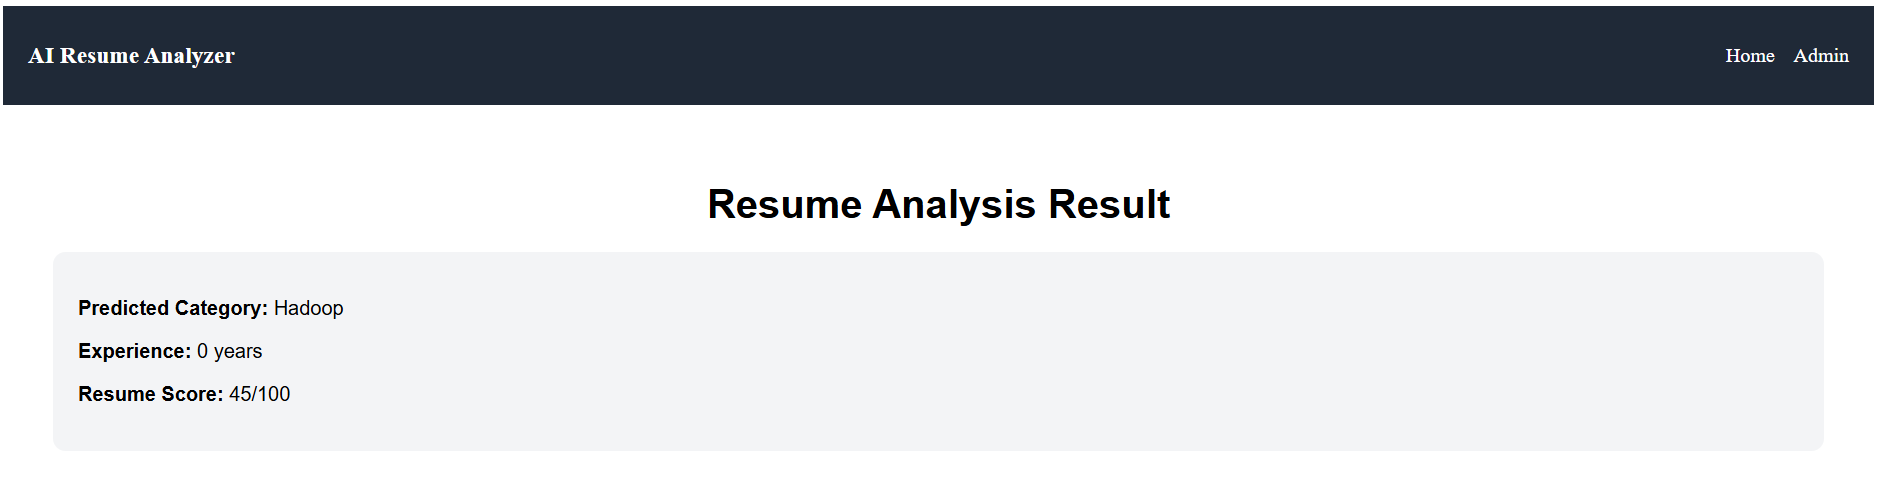
\includegraphics[width=0.8\textwidth]{images/otp21.png}
 \captionof{figure}{ATS Score}
\end{figure}

\begin{figure}[ht]
\centering
 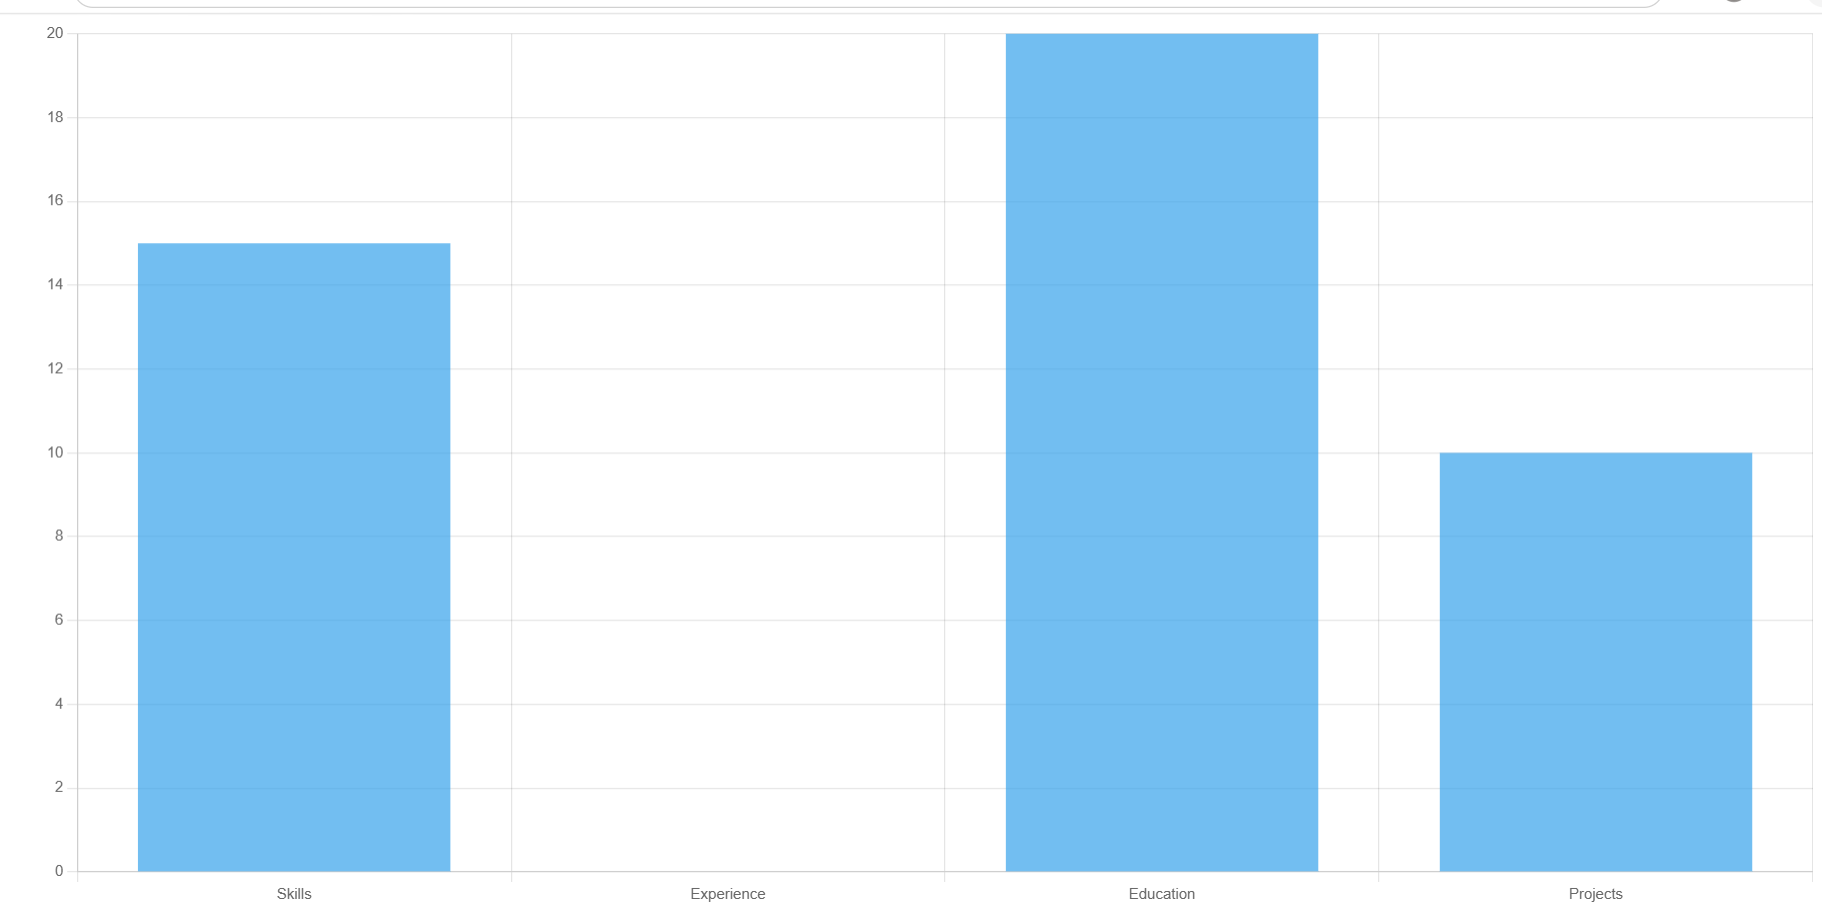
\includegraphics[width=0.8\textwidth]{images/otp22.png}
 \captionof{figure}{Scoring Graph}
\end{figure}

\begin{figure}[ht]
\centering
 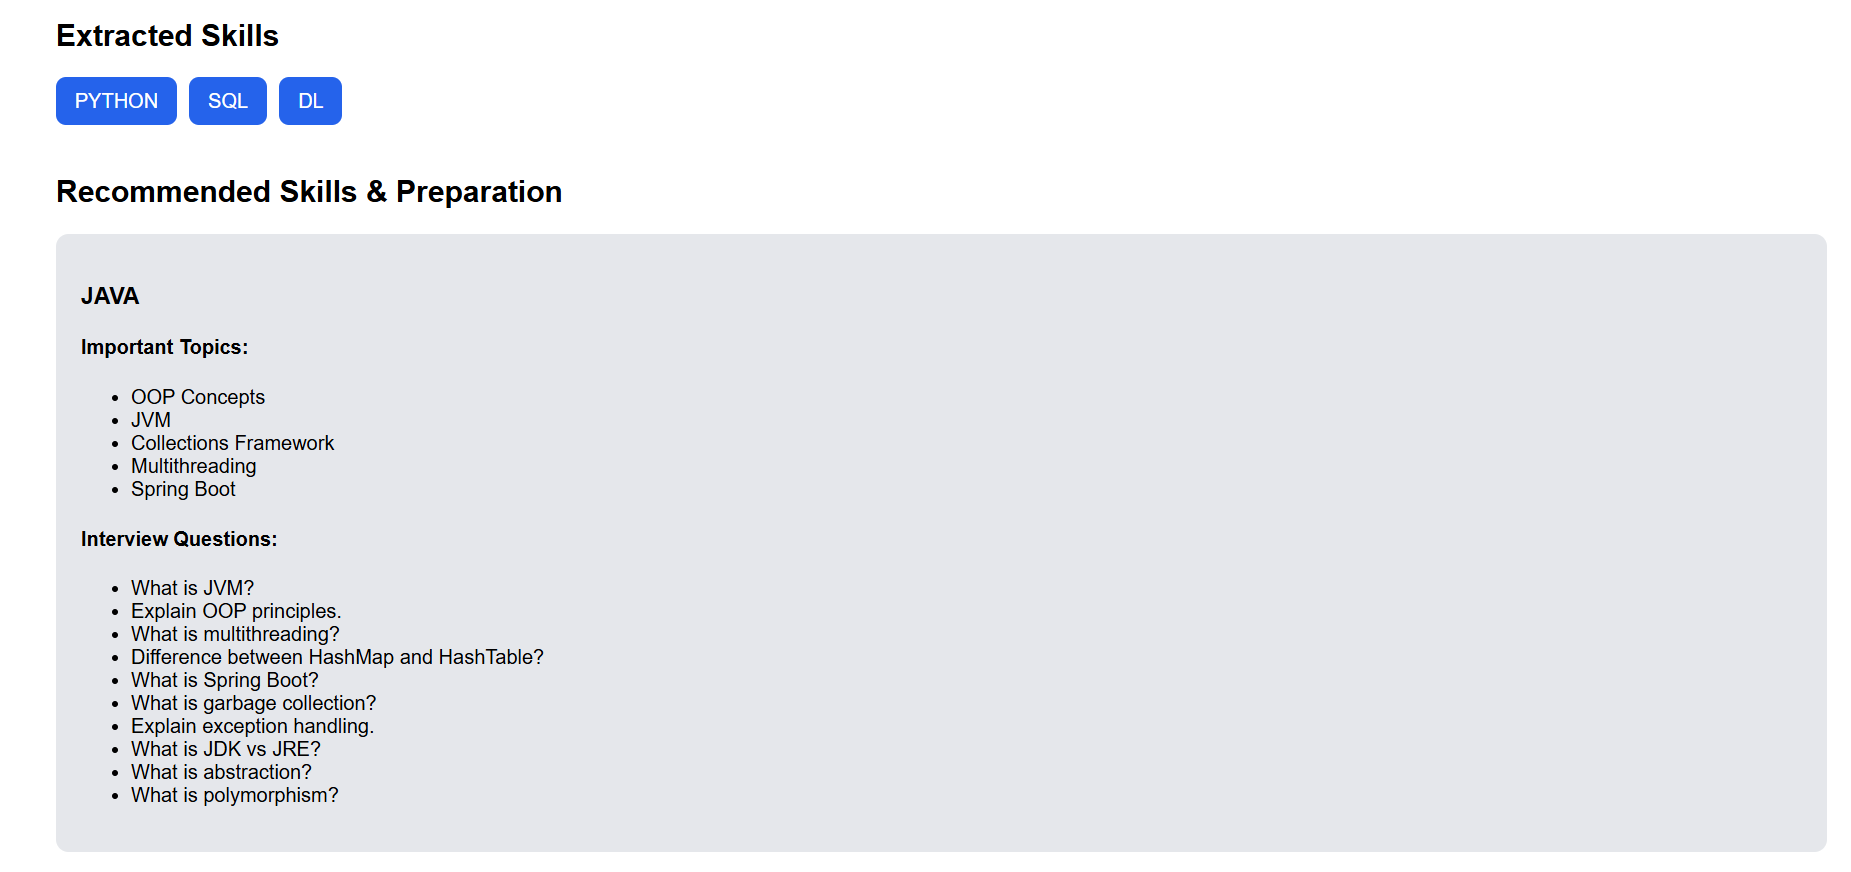
\includegraphics[width=1.0\textwidth]{images/otp23.png}
 \captionof{figure}{Suggetsed Skills}
\end{figure}

\begin{figure}[ht]
\centering
 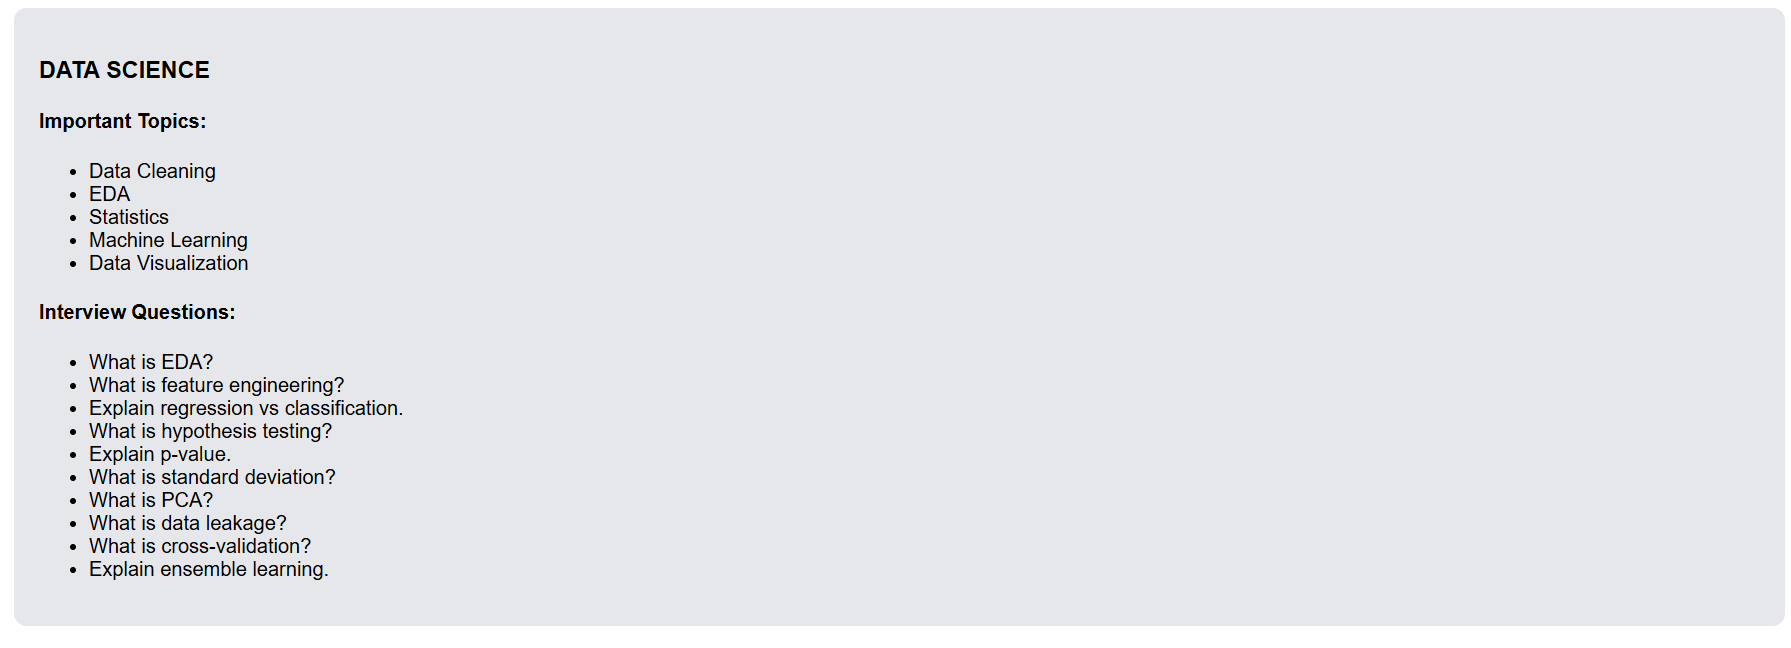
\includegraphics[width=1.0\textwidth]{images/otp24.png}
 \captionof{figure}{Mock Interview Questions}
\end{figure}

\begin{figure}[ht]
\centering
 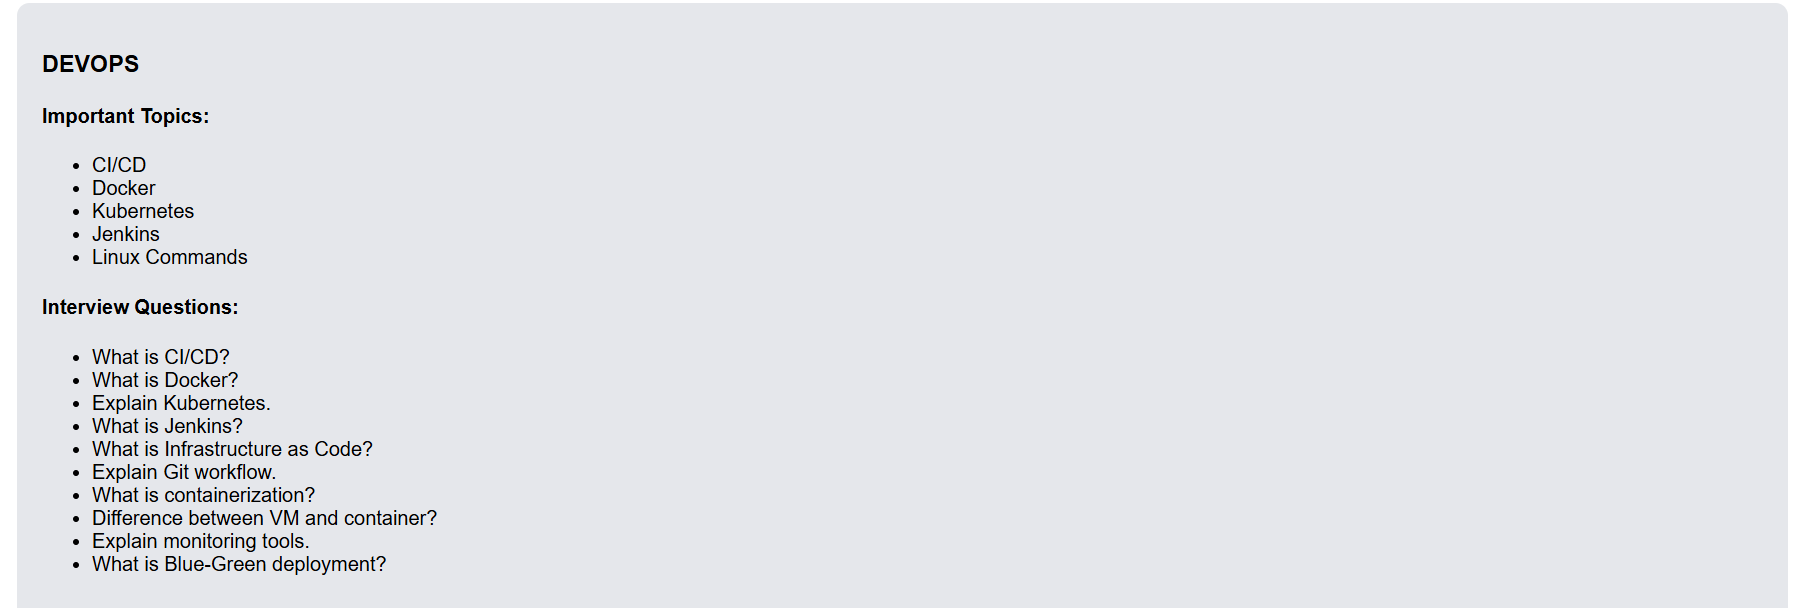
\includegraphics[width=1.0\textwidth]{images/otp25.png}
 \captionof{figure}{Mock Interview Questions}
\end{figure}

\begin{figure}[ht]
\centering
 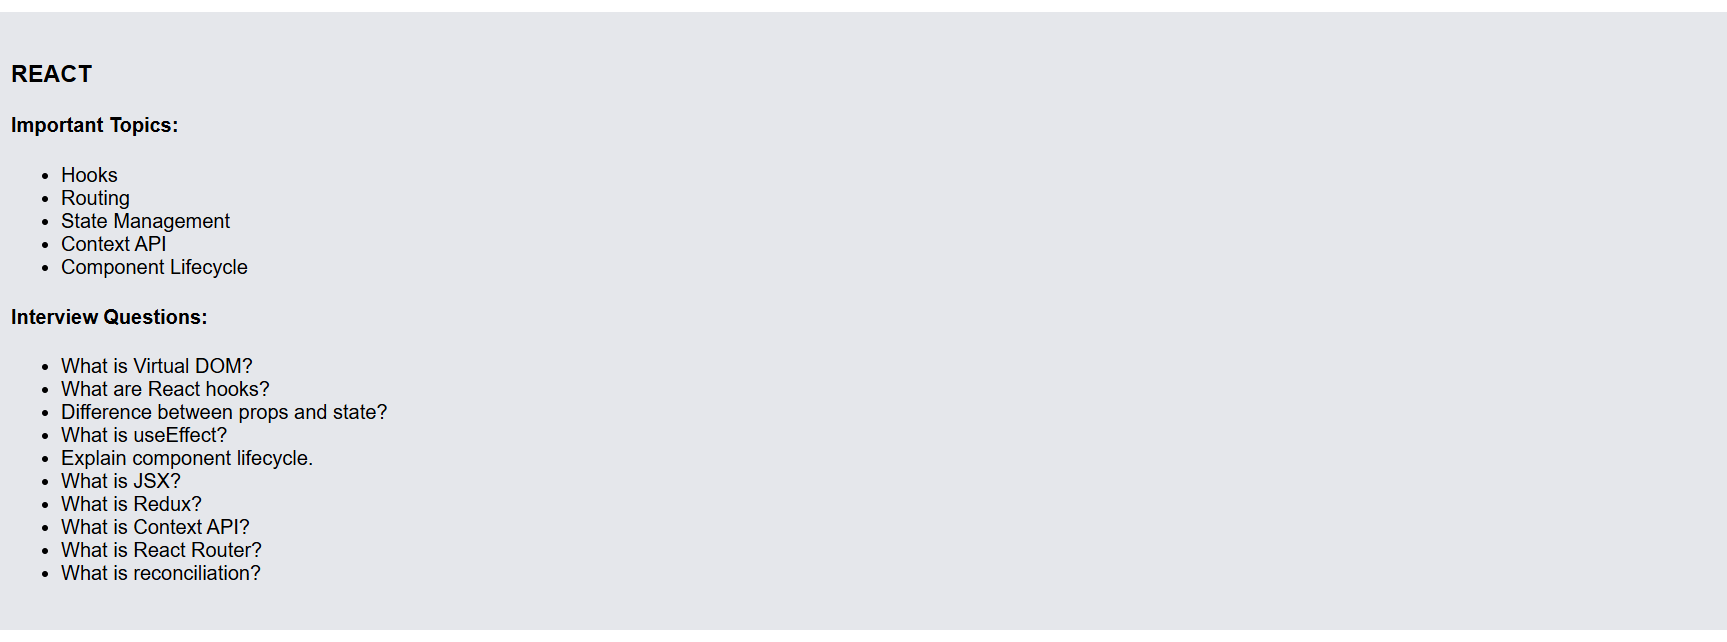
\includegraphics[width=1.0\textwidth]{images/otp26.png}
 \captionof{figure}{Mock Interview Questions}
\end{figure}

\begin{figure}[ht]
\centering
 \includegraphics[width=0.8\textwidth]{images/d_resume.pdf}
 \captionof{figure}{Resume 3}
\end{figure}

\begin{figure}[ht]
\centering
 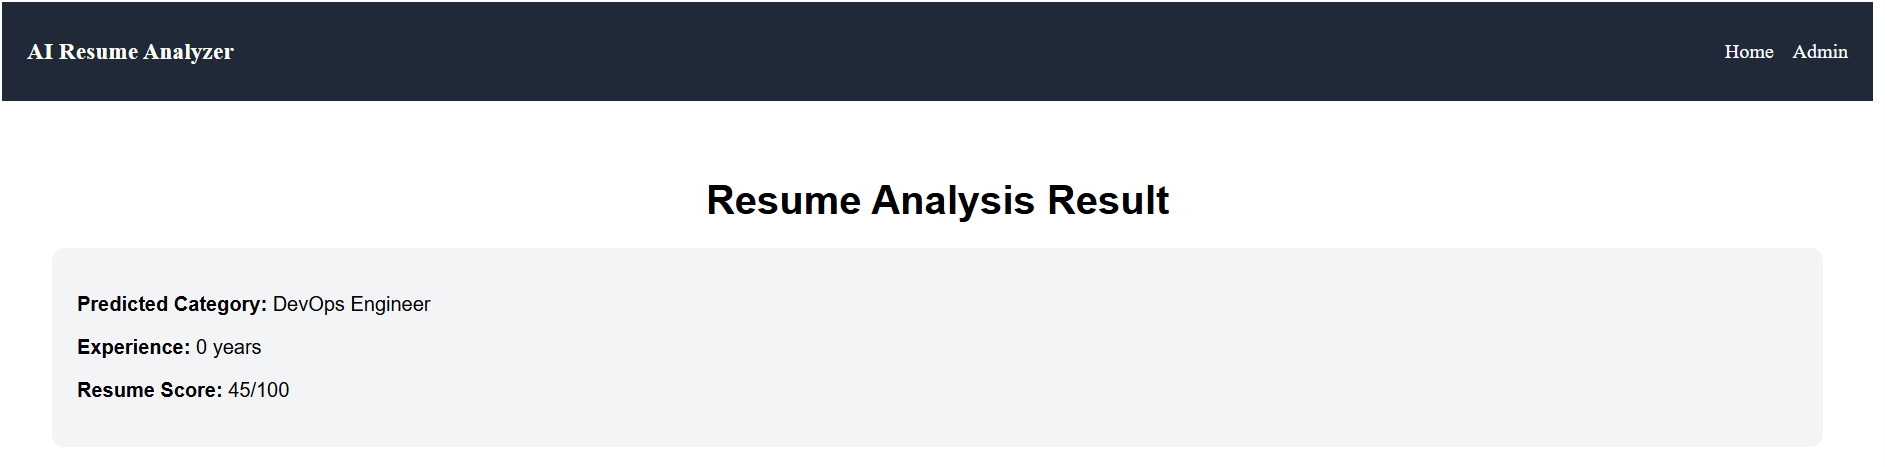
\includegraphics[width=0.8\textwidth]{images/otp31.png}
 \captionof{figure}{ATS Score}
\end{figure}

\begin{figure}[ht]
\centering
 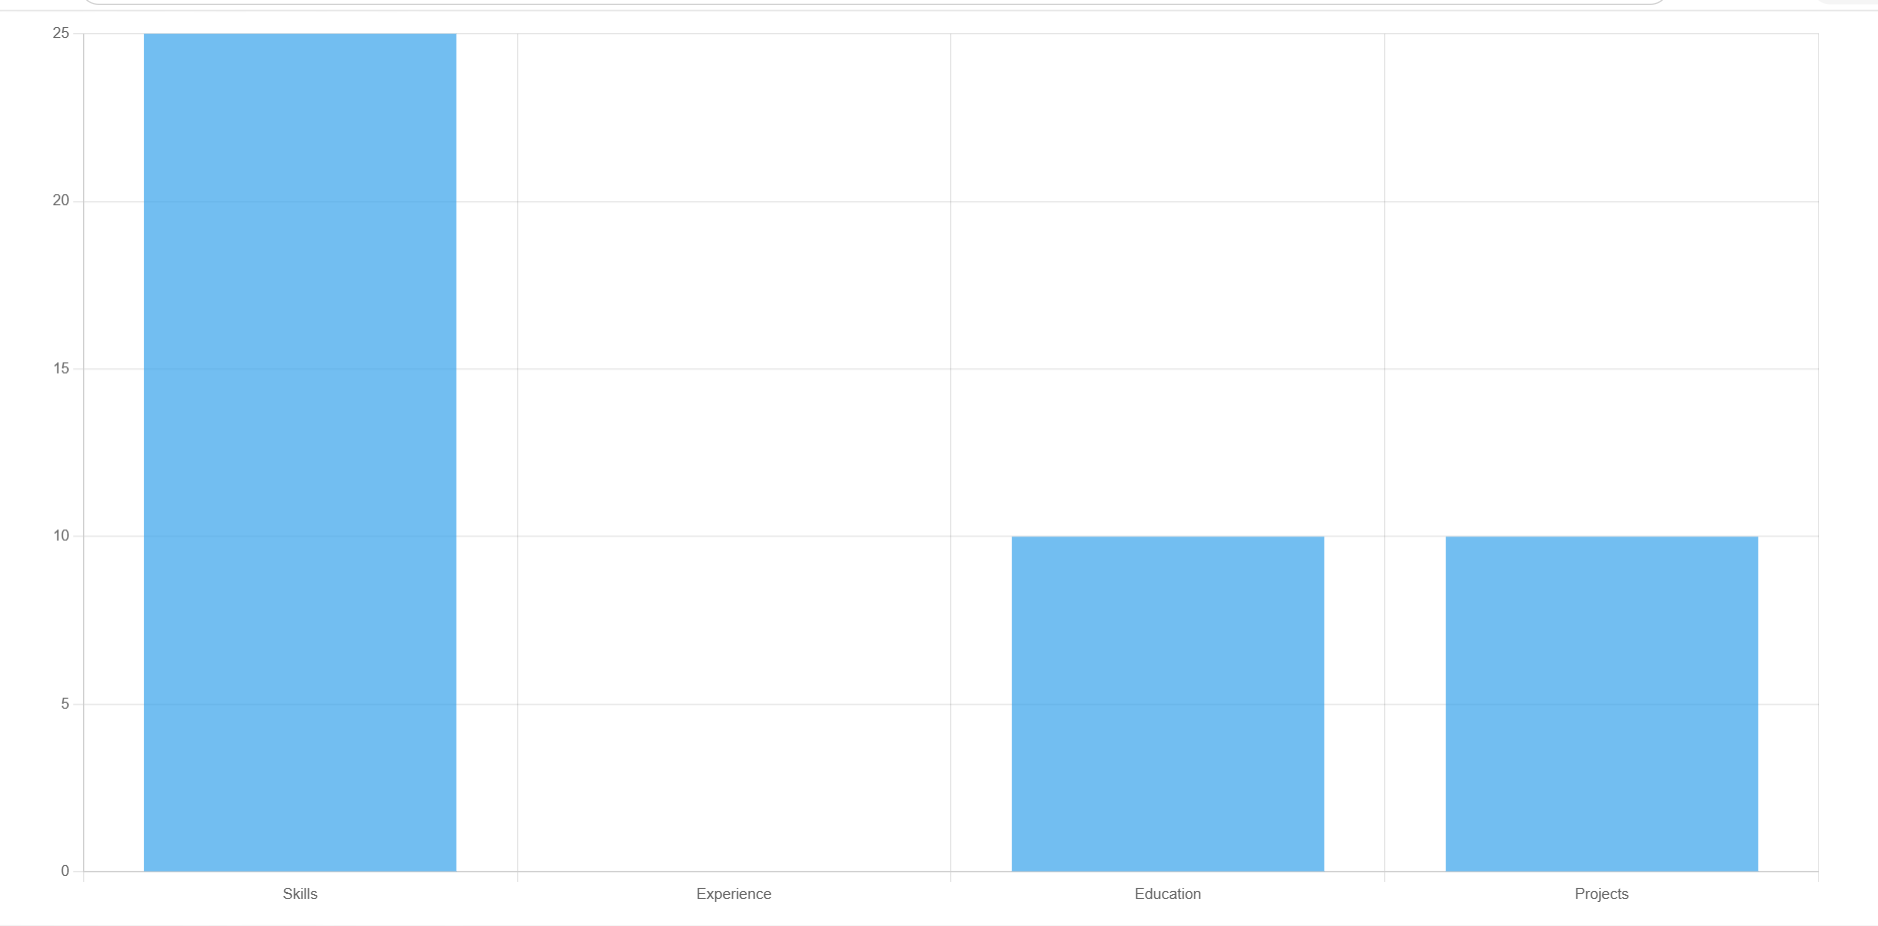
\includegraphics[width=0.8\textwidth]{images/otp32.png}
 \captionof{figure}{Scoring Graph}
\end{figure}

\begin{figure}[ht]
\centering
 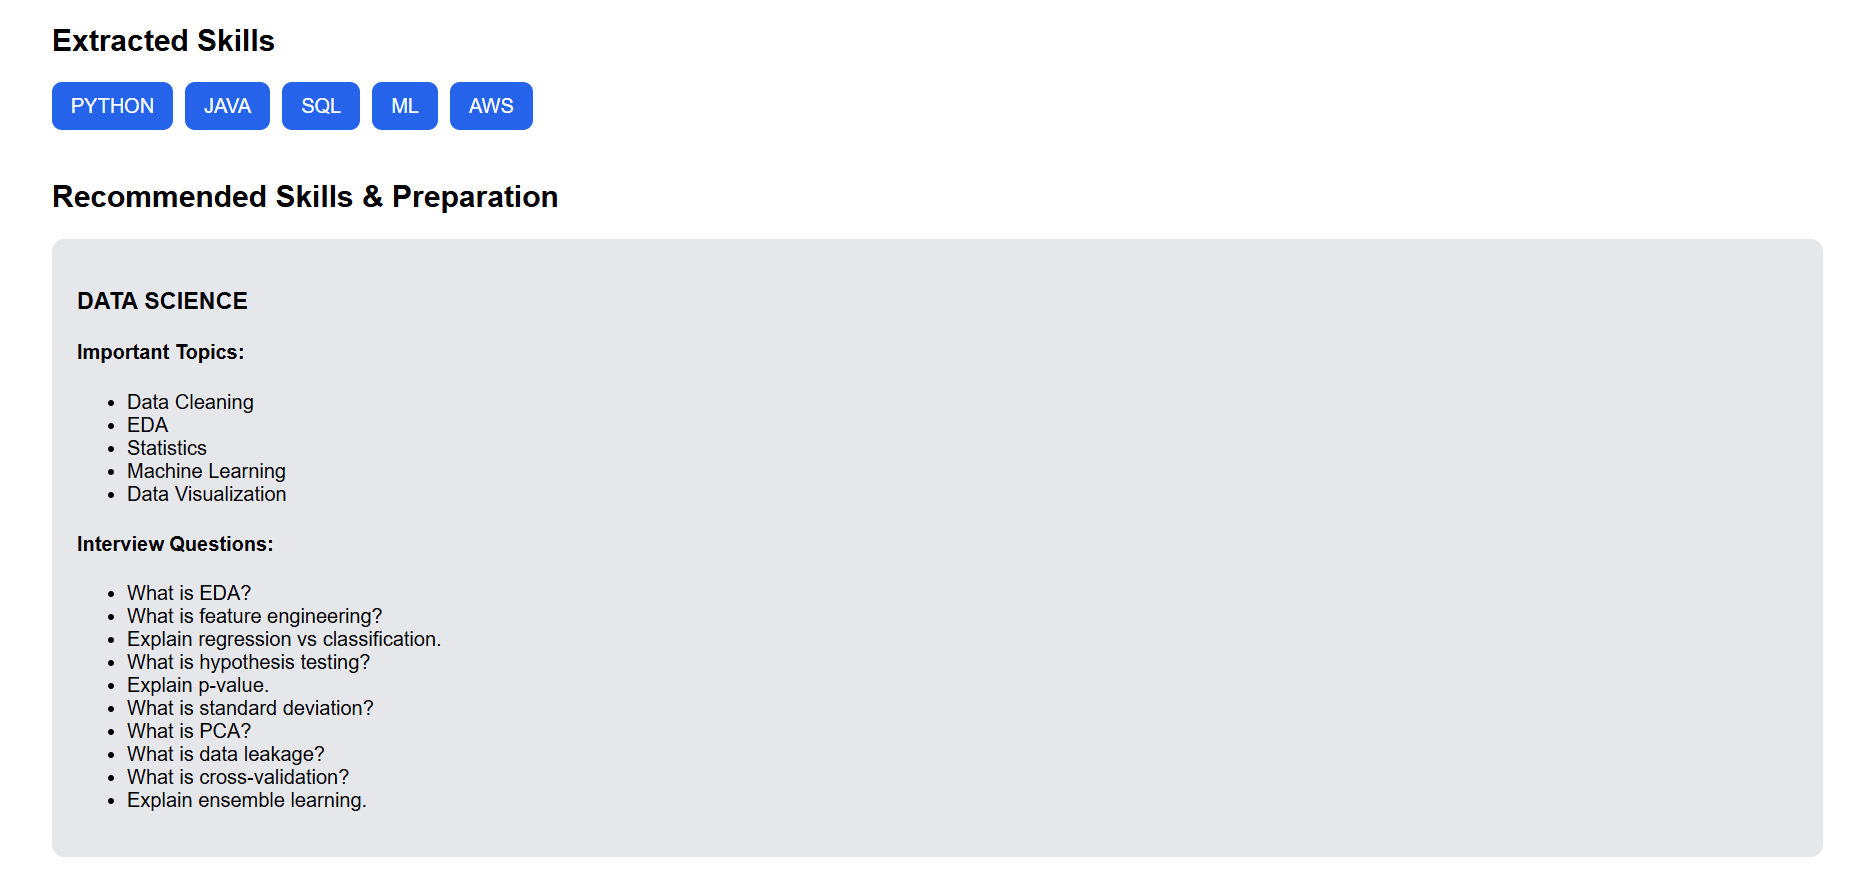
\includegraphics[width=1.0\textwidth]{images/otp33.png}
 \captionof{figure}{Suggetsed Skills}
\end{figure}

\begin{figure}[ht]
\centering
 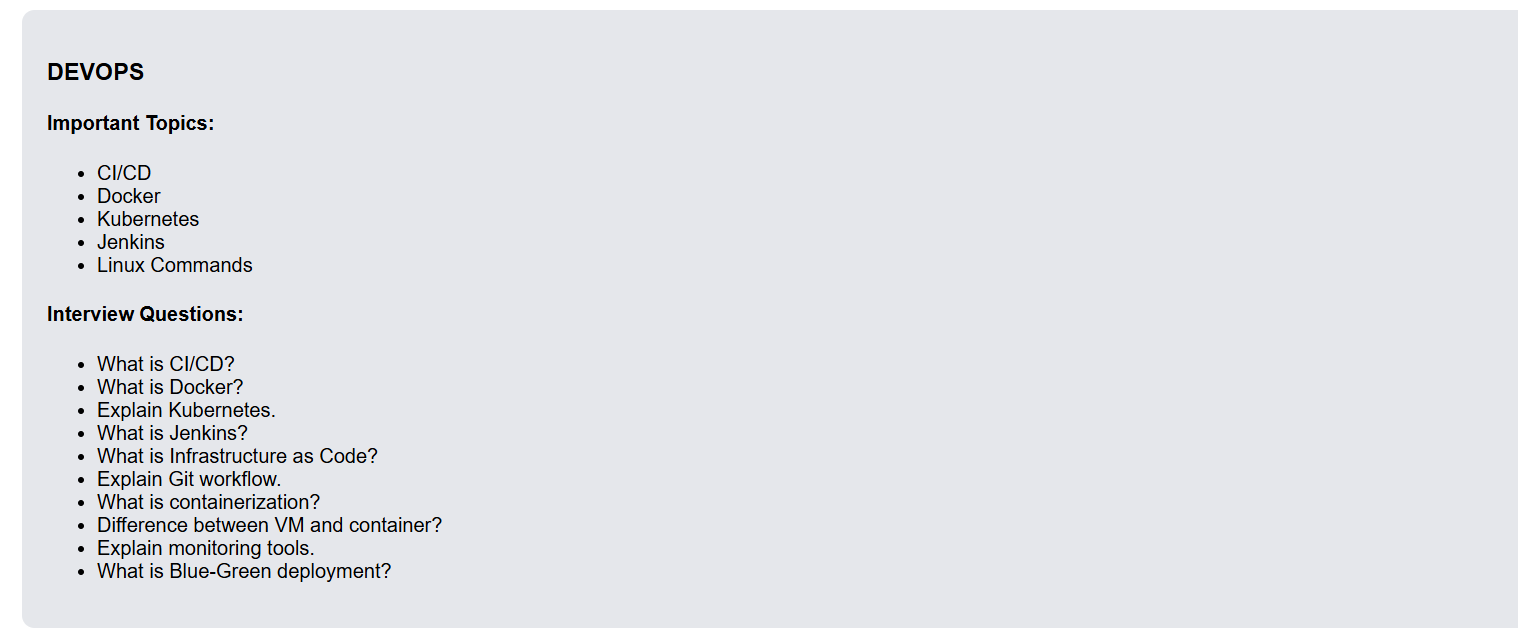
\includegraphics[width=1.0\textwidth]{images/otp34.png}
 \captionof{figure}{Mock Interview Questions}
\end{figure}

\begin{figure}[ht]
%\centering
 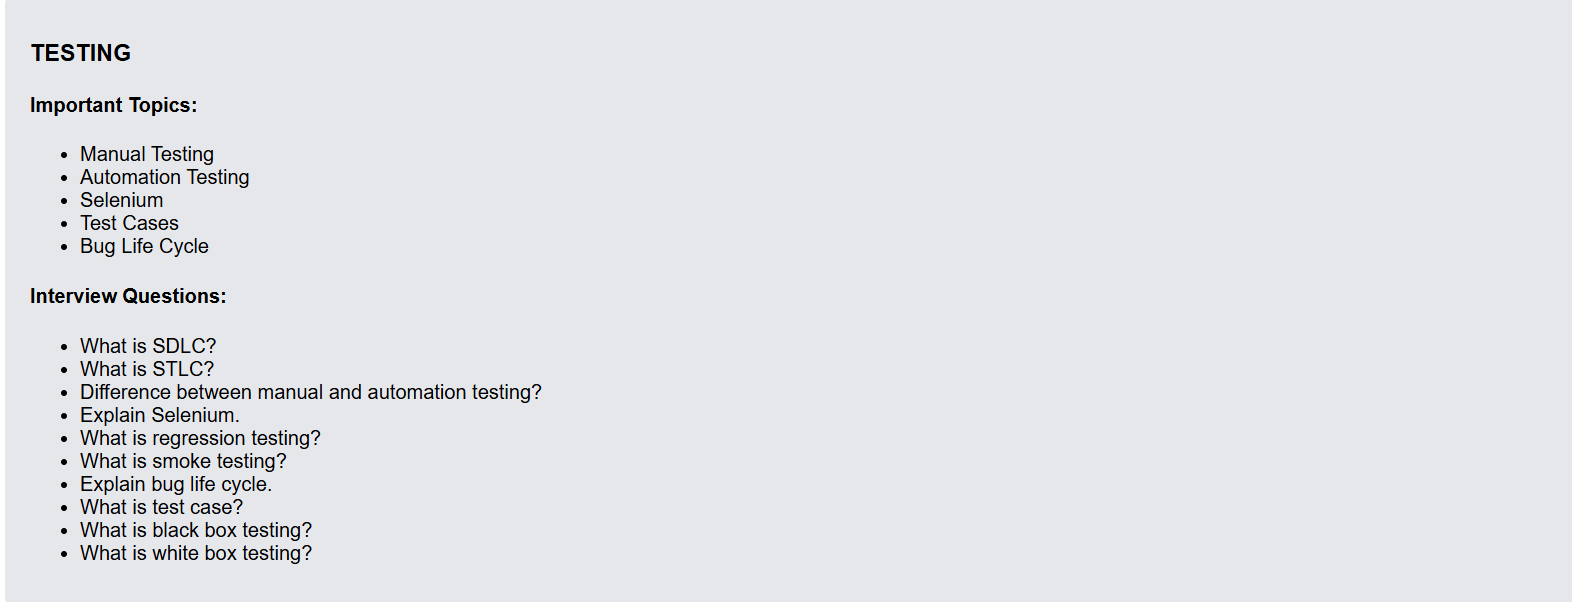
\includegraphics[width=1.0\textwidth]{images/otp35.png}
 \captionof{figure}{Mock Interview Questions}
\end{figure}